%%%%%%%%%%%%%%%%%%%%%%%%%%%%%%%%%%%%%%%%%%%%%%%%%%%%%%%%%%%%%%%%%%%%%%%%%%%%%%%%%%%%%%%%%%%
% Original author of template for CV (Plasmati Graduate CV v1.0 24/03/2013):
%  Alessandro Plasmati (alessandro.plasmati@gmail.com)
% Changes from the template onwards by (latest 30/01/2019):
% Pol del Aguila Pla (poldap@kth.se)
% Changes from the template onwards by (latest 14/02/2020):
% Joaquim Campos (joaquimcampos@duck.com)
% Downloaded from:
%  http://www.LaTeXTemplates.com
% License:
%  CC BY-NC-SA 3.0 (http://creativecommons.org/licenses/by-nc-sa/3.0/)
% Important note (PdaP):
%  This template needs to be compiled with XeLaTeX.
%  The main document font is called Fontin and can be installed in sudo-enabled
%  Linux systems by running fixFONTproblem.sh (will internally call sudo when necessary).
%%%%%%%%%%%%%%%%%%%%%%%%%%%%%%%%%%%%%%%%%%%%%%%%%%%%%%%%%%%%%%%%%%%%%%%%%%%%%%%%%%%%%%%%%%

%----------------------------------------------------------------------------------------
%	PACKAGES AND OTHER DOCUMENT CONFIGURATIONS
%----------------------------------------------------------------------------------------

% Font and paper size
\documentclass[a4paper,11pt]{article}

% Font loading
\usepackage{fontspec}
  \defaultfontfeatures{Mapping=tex-text}
  % Set main font for document
  \setmainfont[SmallCapsFont = Fontin SmallCaps]{Fontin}
\usepackage{bm}

% Formatting
\usepackage{xunicode,xltxtra,url,parskip}

% Coloring
\usepackage[usenames,dvipsnames]{xcolor}

% Margin specification
\usepackage{fullpage}

% Links and other clickable references
\usepackage{hyperref}
  % Link colors
  \definecolor{linkcolour}{rgb}{0,0.2,0.6}
  \hypersetup{colorlinks,breaklinks,urlcolor=linkcolour,linkcolor=linkcolour}

% Costumize section command
\usepackage{titlesec} % Used to customize the \section command
  % Text formatting
  \titleformat{\section}{\Large\scshape\raggedright}{}{0em}{}[\titlerule]
  % Spacing
  \titlespacing{\section}{0pt}{3pt}{3pt}

% Insert images
\usepackage{graphicx}

% Footnotes in tables
\usepackage{footnote}

% Tables that can span several pages
\usepackage{longtable}

% Several biblographies
\usepackage{bibunits}

% Trademark symbol
\usepackage{textcomp}

% enumerations
\usepackage{enumitem}

% Put references sections in the TOC (PDF and HTML links)
\usepackage[nottoc,numbib]{tocbibind}

\def\myname{Joaquim Campos}


\begin{document}

  % Remove page numbers
  \pagestyle{empty}

  %----------------------------------------------------------------------------------------
  %	NAME AND CONTACT INFORMATION
  %----------------------------------------------------------------------------------------

  \begin{center}
    \begin{tabular}{lcr}
	    \par{\centering{\Huge Joaquim \textsc{Campos}}\bigskip\par} & & 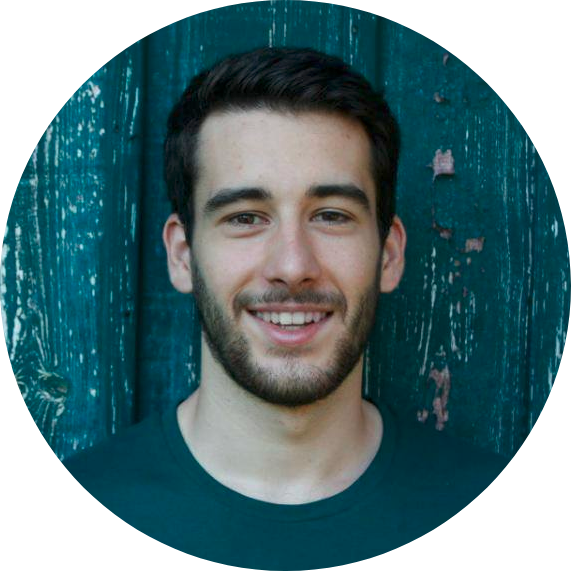
\includegraphics[width=0.3\textwidth]{../../images/Joaquim_circle.png} \\
    \end{tabular}
  \end{center}

  \vspace{16pt}

  \section{Personal data}

    \begin{tabular}{rl}
      \textsc{Address:} & Lisbon, Portugal \\
      % \textsc{Home address:} & Travessa da Cruz da Rocha 3, 4200-344, Porto, Portugal \\
      % \textsc{Mobile phone:} & +351 91-083-2298 \\
      \textsc{Website:} & \url{https://joaquimcampos.com} \\
      \textsc{Email:} & \href{mailto:joaquimcampos@duck.com}{\nolinkurl{joaquimcampos@duck.com}} \\
      \textsc{Others:} & \href{https://scholar.google.com/citations?user=GT-VCroAAAAJ}{Google Scholar} |  \href{https://www.linkedin.com/in/joaquim-campos}{Linkedin} | \href{https://github.com/joaquimcampos/}{Github} \\
    \end{tabular}

  %----------------------------------------------------------------------------------------
  %  Summary
  %----------------------------------------------------------------------------------------

  \vspace{16pt}

  \section{In Brief}
    I am an engineer and researcher specializing in signal processing and artificial intelligence, and I am also a Python developer. In academia, my focus has been on deep learning, learning theory, image and video compression, and inverse problems. Additionally, I co-founded Radiobooks, a startup that assists independent authors and self-learners in automatically converting their books into audiobooks using AI. Through this venture, I have gained knowledge in both product development and DevOps.
    % I am an engineer and researcher specializing in signal processing and artificial intelligence, as well as a Python developer. In academia, I have focused on deep learning, learning theory, image and video compression, and inverse problems. Collaborative research with my colleagues at Disney and EPFL has led to the publication of seven scientific papers, gathering over 300 citations. Additionally, I co-founded Radiobooks, a startup that assists independent authors in automatically converting their books into audiobooks using AI. Through this venture, I gained knowledge of product development and DevOps.
    % Outside the scope of my scientific expertise, I dedicate my time to exploring philosophy, psychology, meditation, ethics, and social systems. I find joy in tackling problems holistically, drawing inspiration from both ancient and modern wisdom, and considering the entire pipeline from philosophical and scientific inquiry to practical application. I appreciate engaging in thoughtful discussions, being exposed to different points of view, and—when suitable—sharing the little I know with others. Currently, I am enroled in a Buddhist philosophy and Meditation course at the Tergar Institute, which will continue on-site between mid-September and mid-December this year (2024).
    % \\
    % \textbf{Highlights} \\
    \\[10pt]
    Highlights:
    \\[-20pt]
    \begin{itemize}[leftmargin=*,noitemsep]
      \item \href{https://www.joaquimcampos.com/pubs.html}{7 publications} with over 300 citations in top-tier venues, and 3 patents.
      \item Contributed to the development of \href{https://www.joaquimcampos.com/compression.html}{pioneering methods} in neural compression.
      \item Crafted \href{https://www.joaquimcampos.com/deepsplines.html}{novel algorithms} for
      % constructing sparse learning models and
      learning the activation functions of a neural network.
      \item Created the \href{https://pypi.org/project/deepsplines/}{"Deep Splines"} PyTorch package.
      \item Co-Founded \href{https://radiobooks.webflow.io/}{Radiobooks}—a startup that makes AI text-to-speech technology.
      \item Built the \href{https://github.com/joaquimcampos/radiobooks-sample}{back-end} of a complex text-to-speech app.
    \end{itemize}

  %----------------------------------------------------------------------------------------
  %	EDUCATION
  %----------------------------------------------------------------------------------------
  \vspace{16pt}

  \section{Education}

    \begin{tabular}{r|p{13cm}}

      % \textsc{\phantom{5}2023 Sep} &
      % %
      % Course in \textbf{Buddhist Philosophy and Meditation}. \\
      % \textsc{Present} &  \footnotesize{\textbf{Tergar Institute}, Kathmandu, Nepal.} \\
      % & \footnotesize{
      %   Head Teacher: Mingyur Rinpoche. Project: \emph{Communicating Madhyamaka Philosophy}. The course will continue on-site between mid-September and mid-December 2024.
      % } \\
      % % 
      % \multicolumn{2}{c}{} \\

      %------------------------------------------------
      \textsc{2020 Feb}  &
      %
      MSc in Communication Systems. \\
      \textsc{2016 Sep} & \emph{Specialization: Signals, Images and Interfaces.} \\
      & \footnotesize{\href{https://www.epfl.ch/en/}{EPFL} (École Polytechnique Fédérale de Lausanne), Lausanne, Switzerland. \newline
      School: \href{https://www.epfl.ch/schools/ic/}{School of Computer and Communication Sciences}.
      } \\
      & \footnotesize{
      % Supervisors and examiner: \textbf{Prof. Michael Unser, Shayan Aziznejad and Prof. François Fleuret}.
      Grade: $\bm{5.67/6.00}$} — Ranking: 2nd/31 \\
      & \footnotesize{
        Focus on signal processing and artificial intelligence. \newline
        % and their applications to imaging and audio
        Master's thesis: \href{https://www.joaquimcampos.com/assets/pubs/MSc_thesis.pdf}{\emph{Higher-Order Regularization Methods for Supervised Learning}}. 
        % Biomedical Imaging Group.
      } \\
      %
      \multicolumn{2}{c}{} \\

      %------------------------------------------------
      \textsc{\phantom{5}2016 Jul} &
      %
      BSc in Electrical and Computer Engineering. \\
      \textsc{2013 Sep} &  \footnotesize{
        \href{https://www.ulisboa.pt/en}{Universidade de Lisboa}, Lisbon, Portugal. \newline
        School: \href{https://tecnico.ulisboa.pt/en/}{Instituto Superior Técnico}.
      } \\
      & \footnotesize{Grade: $\bm{16.4/20.0}$}
    \end{tabular}


  %----------------------------------------------------------------------------------------
  %  WORK EXPERIENCE
  %----------------------------------------------------------------------------------------

  \newpage

  \section{Work experience}

    \begin{tabular}{r|p{13cm}}

      \textsc{2023 Dec} 	& Co-Founder at Radiobooks. \\
      \textsc{2022 Aug} 	& \emph{Converting books into audiobooks automatically using Artificial Intelligence}
      \begin{itemize}[leftmargin=*,noitemsep]
          \item \footnotesize{Designed and built an app for revising AI-generated audio.}
          \item \footnotesize{Our tech stack included Python, FastAPI, MongoDB, Pytest, Docker, GitHub Actions, Codecov, Fly.io, AWS S3, and Better Stack.}
      \end{itemize} \vspace*{-\baselineskip}\\
      \multicolumn{2}{c}{} \\

      %------------------------------------------------

      \textsc{2021 Sep} 	& Research and Teaching Assistant \\
      \textsc{2020 Apr} 	& \emph{Supervised Learning with Sparsity-Promoting Regularization} \\
				& \footnotesize{\href{https://bigwww.epfl.ch/}{Biomedical Imaging Group}, EPFL, Lausanne, Switzerland.
				  }
        \begin{itemize}[leftmargin=*,noitemsep]
          \item \footnotesize{Developed a novel framework to learn the activation functions of a neural network;}
          \item \footnotesize{Designed a spline-based supervised learning method which constructs piecewise-linear models with few regions (sparse).}
        \end{itemize} \vspace*{-\baselineskip}\\
      \multicolumn{2}{c}{} \\

      %------------------------------------------------
      \textsc{2018 Aug} & Research Intern \\
      \textsc{2019 Mar} & \emph{Image and Video Compression using Deep Learning} \\
				& \footnotesize{\href{https://studios.disneyresearch.com/}{Disney Research Studios}, Zurich, Switzerland.}
        \begin{itemize}[leftmargin=*,noitemsep]
          \item \footnotesize{
            Developed the first content-adaptive neural image compression scheme;}
          \item  \footnotesize{
            Aided in the construction of a state-of-the-art neural video compression framework.}
          \end{itemize} \vspace*{-\baselineskip}

    \end{tabular}

  
  %
  %----------------------------------------------------------------------------------------
  %	TEACHING EXPERIENCE
  %----------------------------------------------------------------------------------------

  \vspace{18pt}

  \section{Teaching experience}

    \begin{tabular}{r|p{13cm}}

	  \textsc{Current}     & Teaching assistance in the courses MICRO-310/11: Signals and Systems I/II \\
	  \textsc{2020 Sep} & \footnotesize{\href{https://www.epfl.ch/en/}{EPFL} (École Polytechnique Fédérale de Lausanne), Lausanne, Switzerland.} \\
    & \footnotesize{Taught by Prof. Michael Unser to the \emph{Life Sciences} and \emph{Microenginneering} sections.} \\
    % & \footnotesize{Approximate numbers per semester:
    %           $250$ students;
    %           $65\,\mathrm{h}$ of guidance of exercise sessions and interaction with students on the course forum;
    %           $60\,\mathrm{h}$ of class preparation; and
		% 					$40\,\mathrm{h}$ of exam supervision and grading.
    %           } \\

    \multicolumn{2}{c}{} \\

    \textsc{Current}	 & Supervision of Master semester projects \\
    \textsc{2020 Sep}  & \footnotesize{\href{https://www.epfl.ch/en/}{EPFL} (École Polytechnique Fédérale de Lausanne), Lausanne, Switzerland.} \\
    & \footnotesize{Co-supervisor of two Master semester projects on \href{https://bigwww.epfl.ch/teaching/projects/abstract.html?f=00388}{lipschitz-constrained GANs}.} \\

    \end{tabular}

    %----------------------------------------------------------------------------------------
    % SKILLS
    %----------------------------------------------------------------------------------------

    \vspace{18pt}

    \section{Skills}

    \begin{tabular}{rp{11cm}}
  	Expertise:  & Theoretical and practical aspects of machine learning, deep learning, and signal processing; Python development.
    \vspace{5pt}\\
  	DevOps Experience:       &  \textsc{Python, C, FastAPI, Pytest, PyTorch, CI/CD, Bash, Linux, MongoDB, Docker, Github Actions, Codecov, AWS, Fly.io, Better Stack.}  \vspace{5pt}\\
  	Other skills: 	   & During my academic years, I developed valuable presentation, writing, and teaching skills, much of which I owe to Prof. Michael Unser.
    \end{tabular}

    %----------------------------------------------------------------------------------------
    %	LANGUAGES
    %----------------------------------------------------------------------------------------

    \vspace{18pt}

    \section{Languages}

      \begin{tabular}{rp{10cm}}

        \textsc{Mother tongue:} & Portuguese \\

        \textsc{Professional (C1):} & English \\

        \textsc{Advanced (B2):} & Spanish \\

        \textsc{Conversational (B1):} & French \\

      \end{tabular}

  %----------------------------------------------------------------------------------------
  %	PUBLICATIONS AND PATENTS
  %----------------------------------------------------------------------------------------

  \newpage

  The publications can be consulted \href{https://joaquimcampos.com/pubs.html}{here}. \\[5pt]

  \begin{bibunit}[IEEEtran_Pol]
    \renewcommand\refname{Publications: Science}

    \nocite{
      goujonStableParameterizationContinuous2023,
      aziznejadMeasuringComplexityLearning2023,
      camposLearningContinuousPiecewiseLinear2022,
      bohraLearningActivationFunctions2020,
      aziznejadDeepNeuralNetworks2020,
      djelouahNeuralInterFrameCompression2019,
      camposContentAdaptiveOptimization2019}
    \putbib[../pubs/bibfile]

  \end{bibunit}

  \vspace{20pt}

  \begin{bibunit}[IEEEtran_Pol]
    \renewcommand\refname{Publications: Philosophy}

    \nocite{
      camposMahayanaBuddhistEthicsWork-in-Progress,
      camposWrongnessKillingNonHuman2018} %
    \putbib[../pubs/bibfile]

  \end{bibunit}

  \vspace{20pt}

  \begin{bibunit}[IEEEtran_Pol]
    \renewcommand\refname{Patents}

    \nocite{
      schroersContentAdaptiveOptimization2021,
      schroersSystemsMethodsReconstructing2021,
      schroersSystemsMethodsGenerating2021}
    \putbib[../pubs/bibfile]

  \end{bibunit}

  %----------------------------------------------------------------------------------------
  % INTERESTS AND ACTIVITIES
  %----------------------------------------------------------------------------------------

  % \vspace{-5pt}
  %
  % \section{Interests and activities}
  %
  % \section{On a Personal Note}
  %
  %   I meditate every morning. Cold showers clear my mind. Reader, especially about personal development, philosophy, psychology and society. When I have time a Pixar or Studio Ghibli movie, do Yoga or dancing. Productivity. I shut my cellphone during work and don't touch it on sundays. I practice a vegan lifestyle. I like to think deeply about topics and question my assumptions and beliefs. I work to be a positive influence am mindful of treating others with respect and compassion. I like to have my mind changed and engage in a healthy discussion. I have been fortunate enough to have traveled to abroad every year since I remember. I did competitive volleyball for $10$ years, swimming and represented Portugal at the I represented Portugal at the Youth World Padel Tournament in Mellilla in 2011. Music runs is a passion Piano or Guitar – 4 and 7 years of lessons, respectively.\\
  %
  % \section{Book list}
  %
  % \begin{tabular}{rp{10cm}}
  %
  %   \emph{The Righteous Mind} & by Jonathan Haidt \\
  %
  %   \emph{Animal Liberation} & by Peter Singer \\
  %
  % \end{tabular}
  %
  % \section{Traits}
  %
  % \begin{tabular}{rp{10cm}}
  %
  %   \emph{The Righteous Mind} & by Jonathan Haidt \\
  %
  %   \emph{Animal Liberation} & by Peter Singer \\
  %
  % \end{tabular}

\end{document}
